\documentclass[dvipsnames,tikz]{standalone}
\usepackage{amsmath}
\usepackage{xcolor}
\usepackage{tikz}
\usetikzlibrary{calc}
\usetikzlibrary{decorations.pathreplacing,calligraphy,3d}
\usetikzlibrary{fit, shapes.geometric}

\def\celltower[#1] (#2,#3); {
	\draw[#1, fill=white] (#2,#3) circle (2pt);
	\draw[#1, shift={(#2, #3)}] plot[domain=-0.785:0.785,variable=\t]({0.15*cos(\t r)},{0.15*sin(\t r)});
	\draw[#1, shift={(#2, #3)}] plot[domain=2.356:3.926,variable=\t] ({0.15*cos(\t r)},{0.15*sin(\t r)});
	\draw[#1, shift={(#2, #3)}] plot[domain=-0.785:0.785,variable=\t]({0.25*cos(\t r)},{0.25*sin(\t r)});
	\draw[#1, shift={(#2, #3)}] plot[domain=2.356:3.926,variable=\t] ({0.25*cos(\t r)},{0.25*sin(\t r)});
	\draw[#1, shift={(#2, #3)}] plot[domain=-0.785:0.785,variable=\t]({0.35*cos(\t r)},{0.35*sin(\t r)});
	\draw[#1, shift={(#2, #3)}] plot[domain=2.356:3.926,variable=\t] ({0.35*cos(\t r)},{0.35*sin(\t r)});
}

\begin{document}
	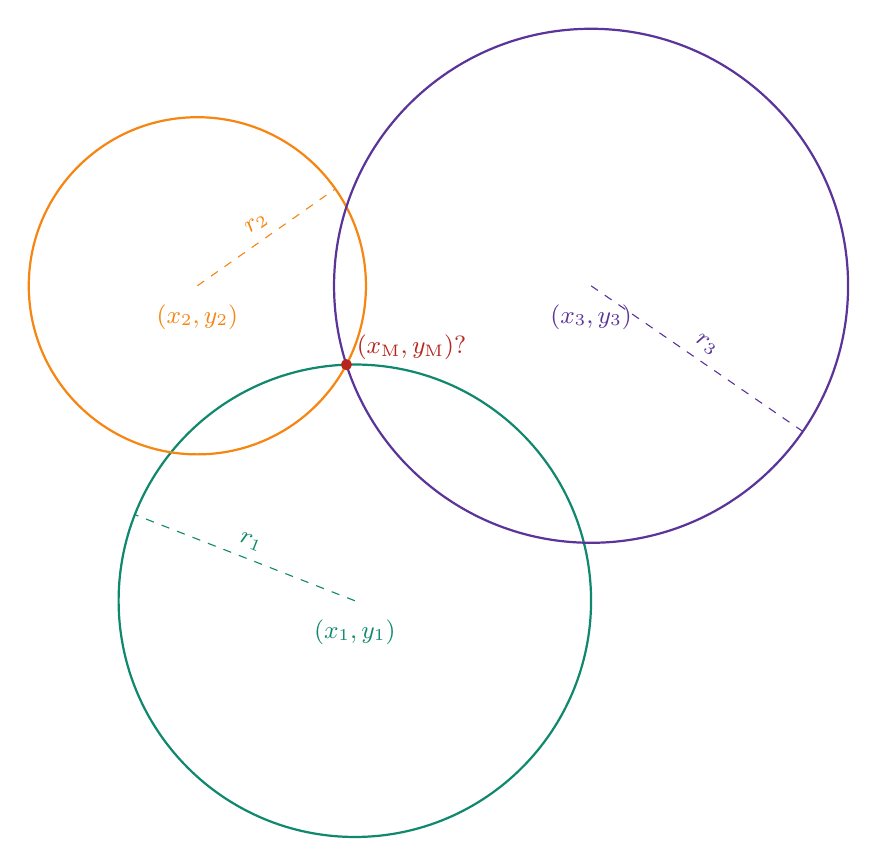
\begin{tikzpicture}[thick, font=\small]
		\draw[PineGreen, dashed, thin] (0,0) to node [sloped, midway, above] {$r_1$} (-2.793,1.093);
		\draw[BurntOrange, dashed, thin] (-2,4) to node [sloped, midway, above] {$r_2$} (-0.25,5.23);
		\draw[RoyalPurple, dashed, thin] (3,4) to node [sloped, midway, above] {$r_3$} (5.69,2.15);		
		
		\draw[PineGreen] (0,0) circle (3.cm);
		\draw[BurntOrange] (-2,4) circle (2.141cm);
		\draw[RoyalPurple] (3,4) circle (3.264cm);
		\celltower[PineGreen] (0,0);
		\celltower[BurntOrange] (-2,4);
		\celltower[RoyalPurple] (3,4);
		
		
		
		\draw[PineGreen] (0,0) node [below,yshift=-3pt] {$(x_1,y_1)$};
		\draw[BurntOrange] (-2,4) node [below,yshift=-3pt] {$(x_2,y_2)$};
		\draw[RoyalPurple] (3,4) node [below,yshift=-3pt] {$(x_3,y_3)$};

		\fill[BrickRed] (-0.107,2.998) circle (2.0pt) node [above right, yshift=-2pt] {$(x_\text{M}, y_\text{M})?$};
	\end{tikzpicture}
\end{document}